\chapter{Introduction}\label{ch:introduction}

\setlength{\epigraphwidth}{0.85\textwidth}
\epigraph{``Il y a une course entre la complexité croissante des systèmes que nous construisons et notre capacité à développer des outils intellectuels pour comprendre leur complexité. Si la course est gagnée par nos outils, les systèmes deviendront finalement plus faciles à utiliser et plus fiables. Sinon, ils continueront à être plus difficiles à utiliser et moins fiables pour tous, sauf pour un ensemble relativement restreint de tâches communes. Étant donné la difficulté de la réflexion, si ces outils intellectuels doivent réussir, ils devront remplacer la pensée par le calcul.''}{\begin{flushright}--Leslie \citet{lamport2002discussion}, \href{https://www.microsoft.com/en-us/research/uploads/prod/2016/12/A-Discussion-With-Leslie-Lamport.pdf}{\textit{Une discussion avec Leslie Lamport}}\end{flushright}}

La complexité du calcul est une telle préoccupation en informatique qu'une grande partie du domaine est consacrée à sa compréhension à travers la lentille de l'analyse des fonctions et de la théorie de l'information. Dans le domaine du génie logiciel, les chercheurs s'intéressent principalement à la complexité de la construction des logiciels, c'est-à-dire la manifestation numérique des algorithmes sur le matériel physique. Un type de complexité logicielle est l'effort cognitif requis pour comprendre un programme. Bien que les logiciels d'aujourd'hui deviennent rapidement plus intelligents, ils ne montrent que peu de signes de devenir plus intelligibles. De meilleurs outils sont nécessaires pour gérer la complexité des systèmes logiciels de construction.

\textit{L'objectif de cette thèse est de développer des méthodes qui réduisent l'effort cognitif nécessaire pour construire des systèmes intelligents, en utilisant des outils de développement, des abstractions de langage de programmation, des tests automatisés et la technologie de virtualisation.}

D'une manière générale, les systèmes intelligents diffèrent des systèmes logiciels ordinaires en ce qu'ils permettent aux machines de détecter des modèles, d'exécuter des tâches et de résoudre des problèmes qu'elles ne sont pas explicitement programmées pour résoudre et que les experts humains étaient auparavant incapables de résoudre en codant en dur des règles explicites. Généralement, ces systèmes sont capables de:\\
%
\begin{enumerate}
\item apprendre des règles généralisables en traitant de grandes quantités de données
\item régler un grand nombre de paramètres libres (des milliers à des milliards)
\item surpasse les humains bien formés dans des tâches spécifiques à un domaine
\end{enumerate}
%
Si l'idée de systèmes intelligents existe depuis des décennies, trois évolutions essentielles ont fait le succès des systèmes intelligents modernes. Premièrement, la puissance de traitement des ordinateurs est devenue plus rapide, moins chère et beaucoup plus facilement disponible. De même, la numérisation de nouveaux ensembles de données a rendu disponibles de vastes quantités d'informations et les coûts de stockage des données ont chuté de façon spectaculaire. (Une clé USB de \$5 a aujourd'hui une capacité de stockage 200 fois supérieure à celle d'un disque dur IBM de 5 MB de 2,000 livres, loué pour \$3,000 par mois en 1956). Plus important encore, a été le développement d'algorithmes d'apprentissage plus efficaces.

Ces dernières années, l'informatique et le génie logiciel ont fait des progrès considérables dans la construction et le déploiement de systèmes intelligents. Presque tous les ordinateurs mobiles du monde sont capables de détecter des objets dans des images, d'effectuer des traductions de la parole au texte et des traductions de langue. Ces percées sont le résultat direct des progrès fondamentaux réalisés dans le domaine des réseaux neuronaux et de l'apprentissage de la représentation. L'adoption de pratiques collaboratives à code source ouvert, dont la communauté du génie logiciel a été la pionnière, a également été la clé du succès des systèmes intelligents modernes. Les ingénieurs en logiciel ont développé des bibliothèques de différenciation automatique comme Theano~\citep{bergstra2010theano}, Torch~\citep{collobert2002torch} et Caffe~\citep{jia2014caffe}, et ont construit de nombreux simulateurs populaires pour l'apprentissage du renforcement. La facilité d'utilisation et la disponibilité de ces outils ont été cruciales pour démocratiser les techniques d'apprentissage approfondi.

Les systèmes intelligents sont largement déployés dans des environnements virtuels comme la science des données et les services en ligne. Mais même avec l'énorme succès des algorithmes d'apprentissage automatique dans des domaines entièrement observables comme la reconnaissance d'images et le traitement de la parole, les systèmes intelligents n'ont pas encore été largement adoptés en robotique (au moment de la rédaction de cette thèse). Ce dilemme peut être partiellement attribué à divers problèmes théoriques tels que l'adaptation au domaine et l'apprentissage par transfert. Pourtant, grâce aux capacités éprouvées des algorithmes d'apprentissage modernes, à l'augmentation exponentielle de la puissance de traitement et aux efforts déployés depuis des décennies pour construire des agents intelligents physiquement incorporés, nous devrions avoir plus de progrès à montrer. Pourquoi cet objectif a-t-il échappé aux chercheurs pendant si longtemps? L'une des raisons, nous le supposons, est le manque d'outils de programmation et d'abstractions pour concevoir, développer, déployer et évaluer les systèmes intelligents. En pratique, ces activités consomment une grande quantité d'efforts cognitifs sans le bon ensemble d'outils et d'abstractions.

Dans le domaine du génie logiciel traditionnel, le modèle Waterfall est un modèle classique de développement de logiciels comprenant différentes étapes~\citep{royce1987managing}. Nous proposons des contributions à quatre étapes: Premièrement, nous faisons la démonstration d'un environnement de développement intégré pour les logiciels de robotique \textit{conception} (\autoref{ch:hatchery}). Ensuite, nous montrons un langage spécifique à un domaine et sans danger pour les programmes différenciables de \textit{implémentation}, un paradigme émergent dans l'apprentissage profond (\autoref{ch:kotlingrad}). Pour \textit{vérifier} cette application, nous utilisons un ensemble de techniques empruntées aux tests basés sur les propriétés~\citep{fink1997property} et à l'apprentissage contradictoire~\citep{lowd2005adversarial} (\autoref{ch:difftest}). Les conteneurs Docker~\citep{merkel2014docker} sont utilisés pour automatiser le \textit{maintenance} d'applications robotiques reproductibles sur des plateformes matérielles hétérogènes (\autoref{ch:ducker}). Enfin, nous présentons quelques remarques de conclusion et les enseignements tirés de la construction de ces outils (\autoref{ch:conclusion}).

%\begin{figure}[H]
%\center
%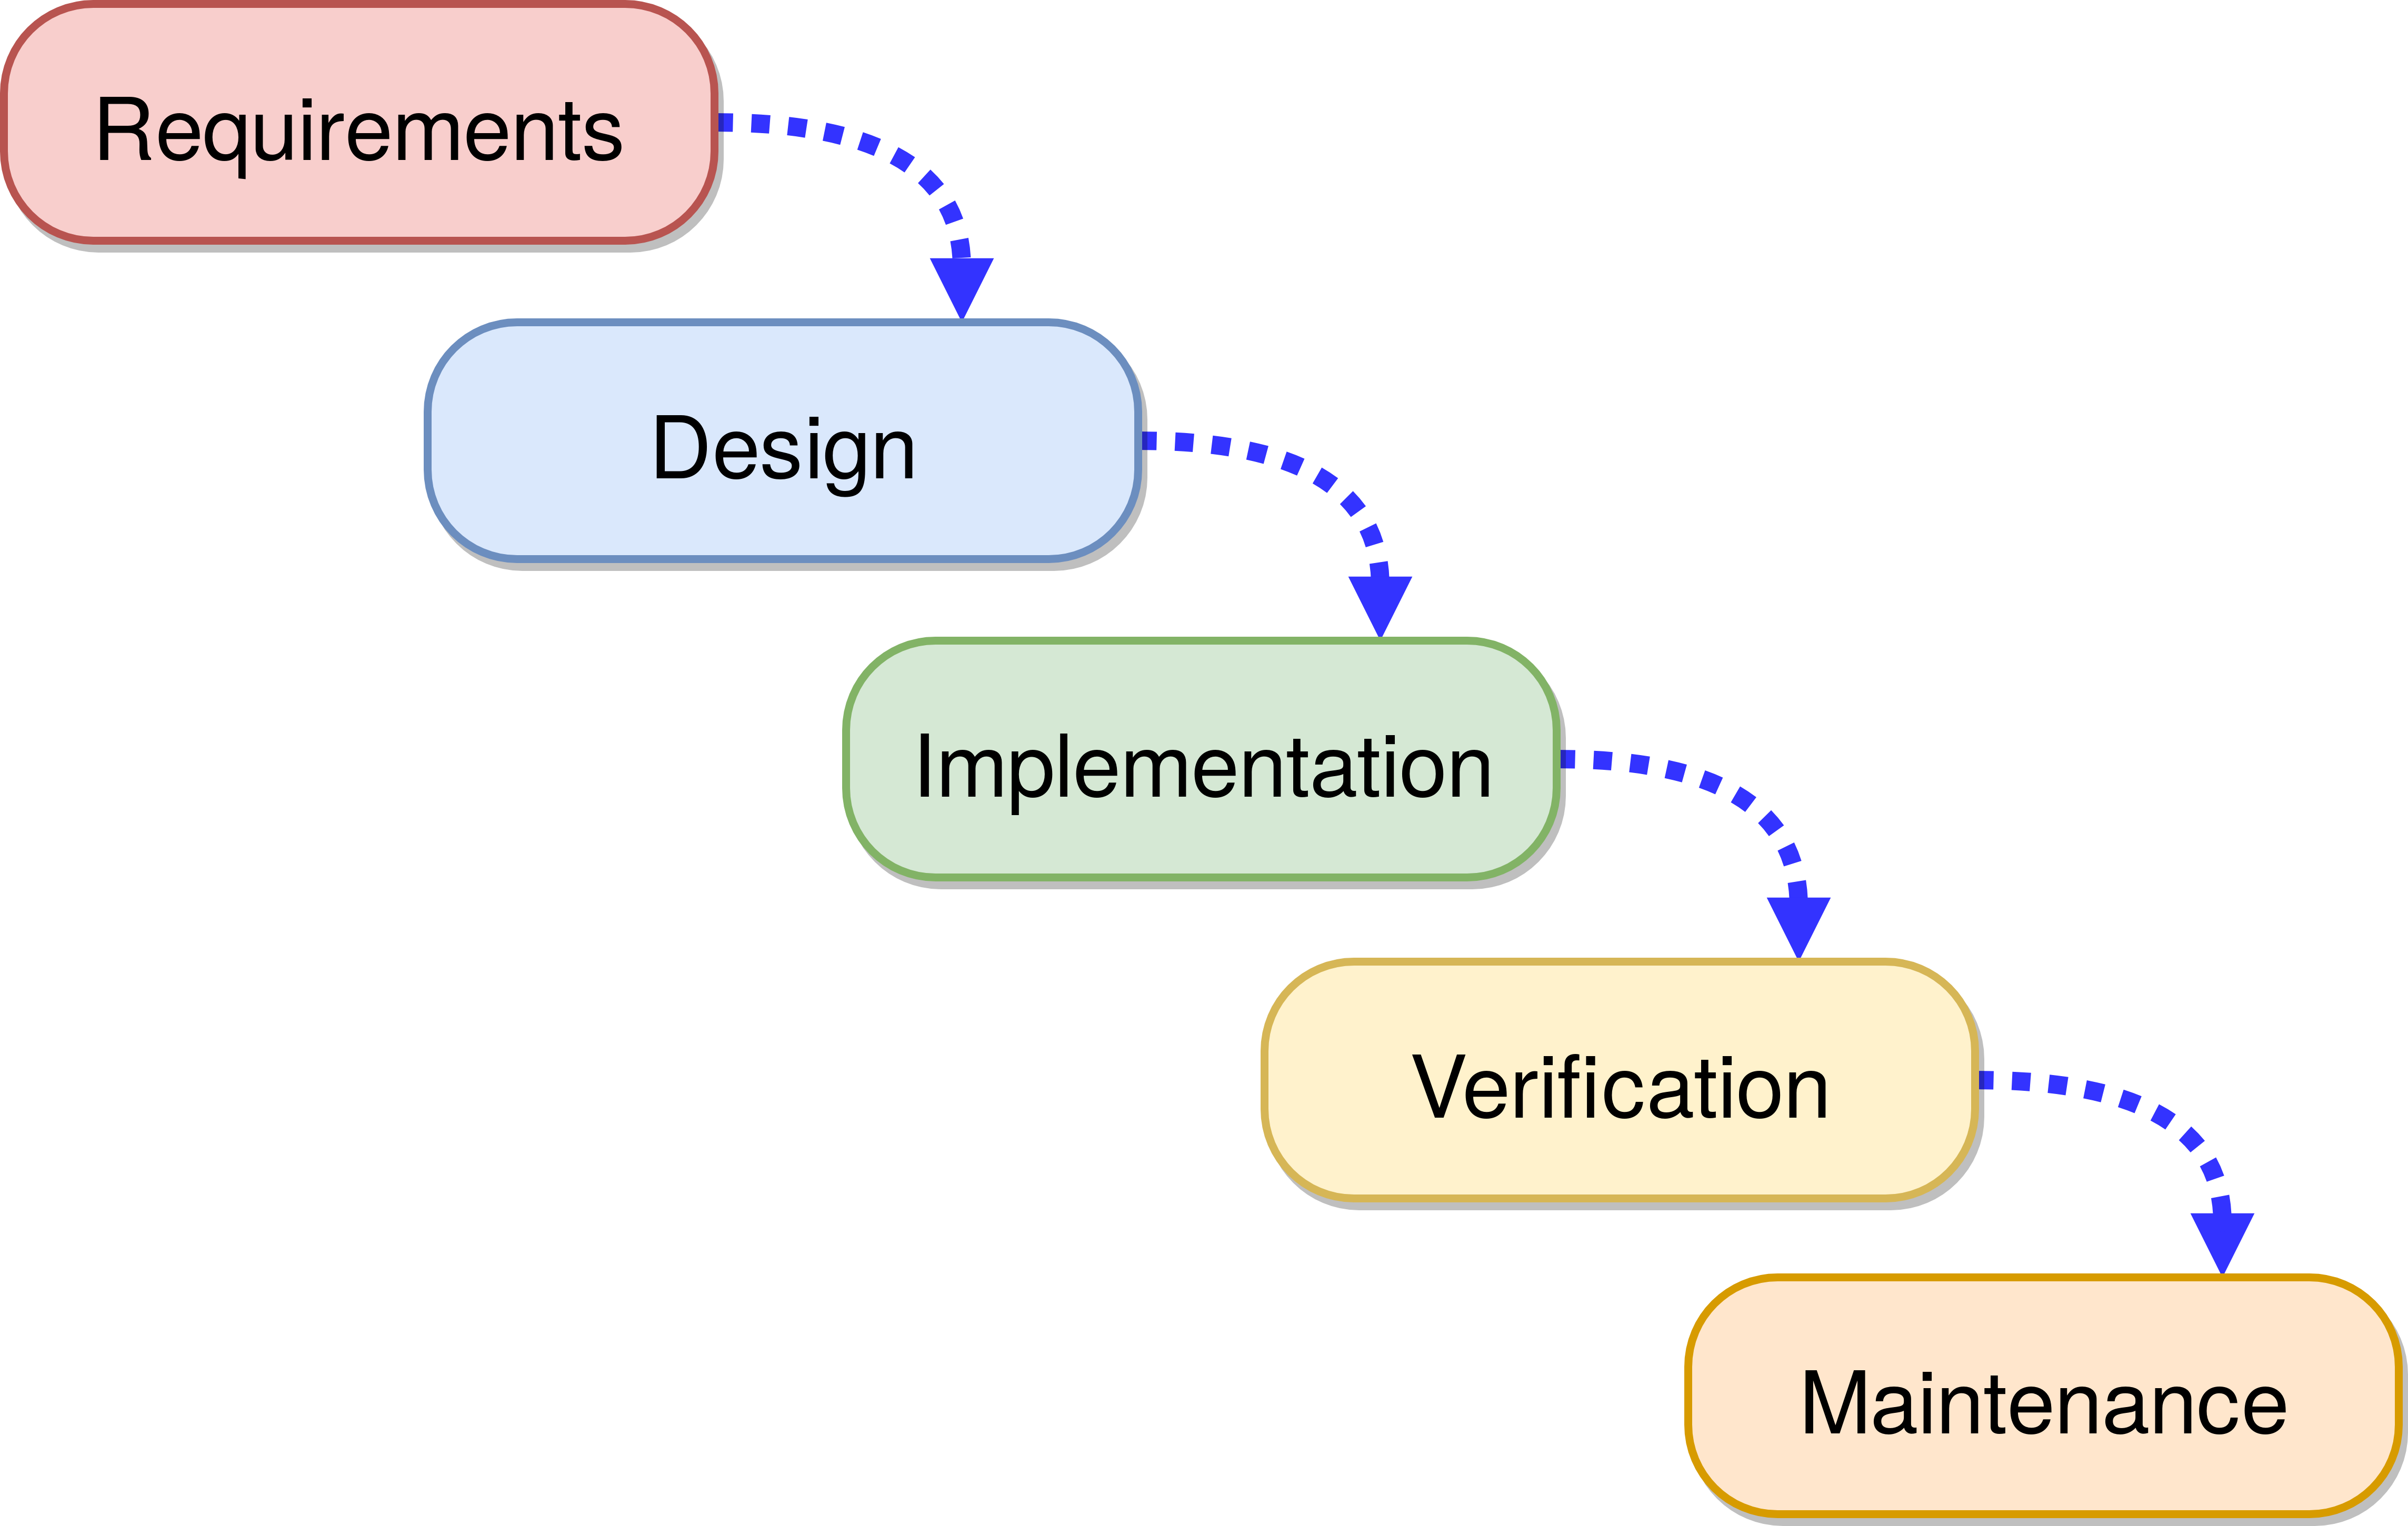
\includegraphics[width=0.70\textwidth]{../figures/waterfall_diagram.png}
%\caption{Le modèle original de cascade de Royce décrit le processus de développement du logiciel. Nous l'utilisons pour guider notre discussion et encadrer nos contributions à l'intérieur de ce modèle.
%\label{fig:waterfall_model}}
%\end{figure}

\section{Conception: Outils de programmation pour la robotique}

Les systèmes logiciels d'aujourd'hui sont des entités profondément complexes. L'époque où un programmeur solitaire, même très compétent, pouvait assurer seul la maintenance d'un grand système logiciel est révolue. Pour mettre efficacement à l'échelle les systèmes logiciels modernes, les programmeurs doivent mettre en commun leur capacité mentale pour former un graphe de connaissances. Les projets logiciels qui reposent sur un petit nombre de responsables ont tendance à disparaître en raison de ce que l'on appelle le "facteur \textit{bus}~\citep{cosentino2015assessing} -- de grandes parties du graphe de connaissances sont enfermées dans la tête de quelqu'un. Les projets logiciels réussis apprennent à distribuer ce graphe et à établir des connexions avec le monde extérieur. Le graphe de connaissances qui s'accumule autour d'un projet logiciel contient des faits, mais aussi des flux de travail pour la programmation, le débogage et la livraison -- des chemins communs à travers le labyrinthe du développement logiciel~\citep{naur1985programming}. Les composants de ce graphique peuvent être engagés à l'écriture, mais la documentation prend du temps et devient périmée avec le temps. Ce qu'il faut, c'est un système qui offre les avantages de la documentation sans les inconvénients de la maintenance.

Le développement de systèmes logiciels comporte un deuxième élément, le graphe social. Le graphe social d'un projet logiciel réussi contient les concepteurs de produits, les gestionnaires et les ingénieurs logiciels qui travaillent de concert pour construire un logiciel bien conçu, cohésif et très performant. Cela implique parfois de réviser la spécification pour tenir compte des défis techniques, ou de réécrire le code source pour supprimer la dette technique. La conception de logiciels est un processus d'optimisation à objectifs multiples et nécessite des collaborateurs ayant un large éventail de compétences et un ensemble d'objectifs communs. Pour produire un logiciel qui se rapproche des critères de ses intervenants, les développeurs sont invités à fournir des prototypes rapides et à intégrer en permanence les commentaires des utilisateurs. Pourtant, les systèmes logiciels d'aujourd'hui sont plus grands et plus compliqués que jamais. Il est donc essentiel de trouver des moyens de collaborer plus efficacement pour construire des systèmes plus intelligents.

Examinons tout d'abord le processus mécanique d'écriture de logiciels à l'aide d'un clavier.

Les environnements de développement intégrés (EDI) peuvent aider les développeurs à créer des applications logicielles complexes en automatisant certaines tâches de programmation répétitives. Par exemple, les EDI effectuent des analyses et des inspections statiques pour détecter rapidement les bogues. Ils permettent de compléter, de remanier et de naviguer dans le code source, et ils automatisent le processus de construction, d'exécution et de débogage des programmes. Bien que ces tâches puissent sembler insignifiantes, leur automatisation promet d'accroître la productivité des développeurs en leur permettant de fournir un retour d'information plus tôt, de détecter les erreurs d'écriture et de libérer des ressources mentales qui pourront être utilisées ailleurs. Plutôt que d'être obligés de se concentrer sur la structure et l'organisation du texte, si les développeurs sont capables de manipuler le code à un niveau sémantique, ils seront beaucoup plus heureux et plus productifs. De plus, en automatisant les tâches mécaniques dans le développement de logiciels, ces outils libèrent l'attention vers l'activité fondamentale de l'écriture et de la compréhension des programmes.

Mais que font réellement les EDI? Ils guident les développeurs à travers le graphe de connaissances d'un projet logiciel. Pensez à ce qu'un nouveau développeur doit apprendre pour se mettre à niveau: en plus d'apprendre le langage, les développeurs doivent apprendre à utiliser des bibliothèques et des cadres (sans doute des langages à part entière). Ils doivent se familiariser avec les outils en ligne de commande pour le développement de logiciels, des outils de construction au contrôle de version et à l'intégration continue. Ils doivent se familiariser avec l'écosystème du logiciel, les styles de programmation, les conventions et les flux de développement. Et ils doivent apprendre à collaborer au sein d'une équipe distribuée de développeurs. En automatisant les tâches courantes dans un environnement de programmation interactif et en rendant explicite la connectivité des graphes grâce au balisage des documents~\citep{goldfarb1981generalized} et à l'édition de projets~\citep{voelter2014towards}, un EDI bien conçu est un outil de traversée de graphes. Il n'est pas surprenant que les EDI soient en fait des bases de données de graphes.

Sous certains aspects, le développement de systèmes intelligents n'est pas différent du génie logiciel classique. Les mêmes principes et meilleures pratiques qui guident le génie logiciel sont également applicables aux systèmes intelligents. Et les mêmes activités, de la conception à la maintenance, continueront à jouer un rôle important dans la construction de systèmes intelligents. Mais à d'autres égards, les outils de programmation génériques utilisés pour développer des logiciels traditionnels nécessiteront des adaptations spécifiques à chaque domaine pour que les systèmes d'apprentissage deviennent des citoyens de premier ordre dans la prochaine génération de logiciels intelligents, notamment dans le cas du développement de la robotique.

Dans ce but, nous avons développé un EDI pour le \href{https://www.ros.org/}{Système d'exploitation des robots} (ROS) appelé \href{https://github.com/duckietown/hatchery}{Hatchery}. Il prend en charge un certain nombre de flux de travail communs pour le développement des ROS, tels que la création de nœuds ROS, l'intégration du simulateur Gazebo, la prise en charge du débogage à distance, l'analyse statique, l'autocomplétion et le refactoring. Dans \autoref{ch:hatchery} nous discutons de la mise en œuvre de ces fonctionnalités et de certains des défis liés à la prise en charge du langage, aux outils de programmation et à l'intégration avec le middleware ROS. Nous soutenons que ces outils réduisent la complexité cognitive de la construction d'applications ROS en adoptant des conventions de codage explicites, en annotant le texte non structuré et en automatisant les tâches de développement répétitives.

\section{Implémentation: Programmation différenciée par type}

Aux premiers temps de l'apprentissage machine, on croyait généralement que l'intelligence à l'échelle humaine émergerait d'une logique de premier ordre suffisamment descriptive. En accumulant une base de données de faits et de leurs relations, les chercheurs pensaient pouvoir utiliser un raisonnement symbolique pour contourner l'apprentissage. Cette approche fondée sur des règles a dominé une grande partie des premières recherches sur l'intelligence artificielle et des efforts considérables ont été consacrés à la création d'ontologies propres à chaque domaine pour saisir les connaissances humaines. Malgré les meilleurs efforts des roboticiens, des ingénieurs en traitement du signal et des chercheurs en langage naturel, les \textit{systèmes experts} n'ont pas pu s'adapter aux applications du monde réel, ce qui a provoqué une grande désillusion dans la recherche sur l'intelligence artificielle pendant plusieurs décennies. Alors que les informaticiens ont sous-estimé la difficulté de l'\textit{apprentissage}, les systèmes experts ont excellé dans des domaines où les systèmes actuels d'apprentissage machine ont du mal à s'adapter, comme le raisonnement classique et l'interprétabilité, et il y a de plus en plus de preuves qui suggèrent que beaucoup de ces idées étaient simplement en avance sur leur temps. Dans notre travail, nous nous inspirons de certains travaux antérieurs sur le raisonnement symbolique~\citep{dwyer1948symbolic, glushkov1971analitik}, les systèmes de types~\citep{lof1973intuitionistic,jay1996shape} et la programmation fonctionnelle~\citep{mccarthy1960recursive, abelson1996structure}.

Ce qui a finalement été montré à l'échelle, c'est l'idée de l'apprentissage connexionniste. En imbriquant des approximateurs de fonctions aléatoires, appelés perceptrons, et en mettant à jour les paramètres libres à l'aide de la rétropropagation~\citep{werbos1990backpropagation, rumelhart1988learning}, le système résultant est capable d'apprendre une quantité surprenante de comportements intelligents. L'approche, appelée réseaux neuronaux artificiels (ANN), remonte au milieu du 20ème siècle~\citep{ivakhnenko1965cybernetic, rosenblatt1958perceptron}, mais n'a été pleinement réalisée in silico qu'après la généralisation de l'informatique bon marché et des grands ensembles de données~\citep{lecun2015deep}. En théorie, une seule couche d'imbrication est capable d'approcher toute fonction différentiable continue~\citep{hornik1989multilayer}, mais en pratique, l'apprentissage nécessite de composer de nombreux approximateurs de ce type de manière profondément imbriquée, d'où le terme, \textit{deep neural networks} (DNNs). L'importance de la profondeur a été soupçonnée pendant de nombreuses années, mais l'algorithme de rétropropagation original avait des difficultés à former les DNN en raison du problème du gradient de disparition~\citep{bengio1994learning}. La résolution de ce problème a nécessité un certain nombre d'adaptations et de nombreuses années pour être entièrement débogué. Ce n'est que vers 2013 que l'apprentissage approfondi est devenu compétitif par rapport aux experts humains dans des domaines spécifiques.

Bien qu'il ait fallu une recherche fondamentale en matière d'apprentissage approfondi pour réaliser le plan connexionniste, le succès de l'apprentissage approfondi moderne peut être en partie attribué aux outils logiciels de calcul des dérivés mathématiques, une étape clé de l'algorithme de rétropropagation. Bien qu'il n'ait pas encore été établi si et comment les dérivés peuvent être calculés dans les circuits biologiques, les dérivés sont essentiels pour la formation des ANN. Pendant de nombreuses années, la forme symbolique de ces dérivés a été dérivée analytiquement lors du prototypage d'une nouvelle architecture de réseau neuronal, un processus fastidieux et sujet aux erreurs. Il existe un algorithme bien connu dans la communauté du calcul scientifique qui remonte aux années 1970, appelé \textit{différenciation automatique} (AD)~\citep{linnainmaa1970representation, griewank1989automatic}, qui est capable de calculer des dérivés pour des fonctions différentiables arbitraires. Mais étonnamment, ce n'est que beaucoup plus tard, après le développement de Theano~\citep{bergstra2010theano}, que l'AD a été largement adopté par la communauté de l'apprentissage machine. Cette bibliothèque a considérablement accéléré le rythme de la recherche sur l'apprentissage profond et a stimulé le développement d'autres cadres AD comme TensorFlow~\citep{abadi2016tensorflow} et PyTorch~\citep{paszke2019pytorch}.

Les systèmes intelligents conçus doivent réfléchir attentivement aux langages et aux abstractions. Si les développeurs doivent mettre en œuvre la rétropropagation à la main, ils auront peu de temps pour réfléchir aux caractéristiques de haut niveau de ces systèmes. De même, si les abstractions de programmation sont trop spécifiques, de petites variations nécessiteront une réimplémentation coûteuse. Cela n'est pas différent du génie logiciel traditionnel - en tant qu'ingénieurs, nous devons choisir les bonnes abstractions pour la tâche à accomplir. Trop bas niveau et la conception se perd dans les détails -- trop abstrait et les détails se perdent complètement. Avec un apprentissage approfondi, la nécessité de choisir de bonnes abstractions est encore plus importante, car la relation entre le code source et le comportement est déjà difficile à déboguer, en raison de la complexité des réseaux de neurones et de la programmation des tableaux. Une composante de cette complexité se trouve dans le système de types.

La plupart des cadres AD existants pour l'apprentissage machine sont écrits dans des langages à typage dynamique comme Python, Lua et JavaScript, avec quelques premières implémentations, notamment des projets comme \href{http://deeplearning.net/software/theano/}{Theano}~\citep{bergstra2010theano}, \href{http://torch.ch/}{Torch}~\citep{collobert2002torch} et \href{https://caffe.berkeleyvision.org/}{Caffe}~\citep{jia2014caffe}. Des idées similaires sont apparues dans des langages fonctionnels à caractères statiques, tels que Java (\href{https://github.com/uniker9/JAutoDiff}{JAutoDiff}~\citep{nureki2012jautodiff}, \href{https://deeplearning4j.org/}{DL4J}~\citep{team2016dl4j}, \href{https://github.com/Hipparchus-Math/hipparchus}{Hipparchus}~\citep{andrea2016automatic}), Scala (\href{https://tongfei. me/nexus/}{Nexus}~\citep{chen2017typesafe}), F\# (\href{http://diffsharp.github.io/DiffSharp/}{DiffSharp}~\citep{baydin2015diffsharp}), \href{https://www. tensorflow.org/swift}{Swift}~\citep{lattner2018tensorflow}, Haskell (\href{https://github.com/leopiney/tensor-safe}{TensorSafe}~\citep{pineyro2019structure}) et al, mais peu d'entre eux sont capables de vérifier la forme des tableaux multidimensionnels dans leur système de types, et ceux qui le font sont implémentés dans des langages expérimentaux avec des types dépendants. Dans notre travail, nous démontrons la viabilité de la vérification de type dans un langage largement utilisé. Cela garantit que les programmes sur les matrices, s'ils se compilent, ont la forme correcte et peuvent être évalués numériquement au moment de l'exécution.

\href{https://github.com/breandan/kotlingrad/}{Kotlin$\nabla$} est un langage dédié interne (eDSL) pour la programmation différenciable dans un langage appelé \href{https://kotlinlang.org}{Kotlin}, un langage de programmation à caractères statiques prenant en charge la programmation asynchrone et la compilation multi-plateforme. Dans Kotlin$\nabla$ (\autoref{ch:kotlingrad}), nous décrivons une implémentation algébrique de la différenciation automatique avec des opérations de tenseur de type sécurisé. Notre approche diffère de la plupart des cadres AD existants dans la mesure où Kotlin$\mathbf{\nabla}$ est la première bibliothèque de type sécurisé AD à entièrement compatible avec le système de type Java, ne nécessitant aucune métaprogrammation, réflexion ou intervention du compilateur pour être utilisée.

\section{Vérification: Tester les systèmes intelligents}

La plupart des phénomènes naturels, en particulier ceux liés à la vision, à la planification et à la locomotion, sont des créatures de grande dimension. Richard Bellman a célèbremment appelé ce problème la "fléau de la dimensionnalité". Notre univers physique est peuplé de problèmes simples à poser, mais apparemment impossibles à résoudre en son sein. Claude Shannon, un contemporain de Bellman, a calculé que le nombre de parties d'échecs uniques dépassait $10^{120}$, soit plus que le nombre d'atomes dans l'univers d'environ quarante ordres de grandeur~\citep{shannon1950chess}. À l'époque, on pensait que de tels problèmes seraient insurmontables sans percées fondamentales dans les algorithmes et les machines informatiques. En effet, si Bellman ou Shannon n'ont pas vécu pour voir le jour, il n'a fallu qu'un demi-siècle de progrès en informatique~\citep{campbell2002deep} avant que des solutions à des problèmes du même ordre de complexité, découverts pour la première fois lors de l'explosion cambrienne il y a 541 millions d'années, soient mises en œuvre avec une marge concurrentielle sur les ordinateurs modernes~\citep{pratt2015cambrian}.

Alors que l'informatique a fait d'énormes progrès dans la résolution des cas les plus courants, le fléau de la dimensionnalité de Bellman hante toujours la longue queue de l'apprentissage machine, en particulier des distributions très dispersées. Comme la dimensionnalité de nombreuses fonctions du monde réel que nous voudrions approcher est d'une ampleur insurmontable, il est difficile de vérifier le comportement d'une solution candidate dans tous les régimes, en particulier dans des contextes où les échecs sont rares mais catastrophiques. Selon certaines études, les conducteurs humains comptent en moyenne 1,09 décès par cent millions de miles~\citep{kalra2016driving}. Un nouveau logiciel pour un véhicule autonome devrait accumuler 8,8 milliards de miles de conduite afin d'approcher le taux de mortalité d'un conducteur humain à 20\% près avec un intervalle de confiance de 95\%. Le déploiement d'un tel système dans le monde réel serait problématique sur le plan logistique, sans parler de l'éthique.

D'un point de vue réaliste, les systèmes intelligents ont besoin de meilleurs moyens de mettre en pratique leurs compétences et de sonder l'efficacité d'une solution candidate dans le cadre d'un budget de calcul limité, sans nuire aux humains dans le processus. L'objectif de ces tests est de mettre en évidence les erreurs, mais aussi, en fin de compte, de fournir un retour d'information au système. Dans le domaine du génie logiciel, le véritable système testé est l'écosystème des humains et des machines qui se fournissent mutuellement des moyens de subsistance. Le succès de cet arrangement dépend d'un mécanisme de test externe pour appliquer une barre de rigueur minimale, généralement une forme de test matériel ou humain en boucle. Si le mécanisme de test n'est pas opposé d'une manière ou d'une autre au système testé, un système intelligent peut se tromper, ce qui n'est ni dans l'intérêt du système ni dans celui de ses utilisateurs.

Plus largement, nous pouvons considérer la vérification de type (\autoref{ch:kotlingrad}) et les tests automatisés (\autoref{ch:difftest}) comme faisant partie d'un ensemble d'outils plus large pour la vérification et la validation des logiciels. Plus les anomalies sont détectées rapidement, plus elles sont faciles à corriger et plus les systèmes autonomes peuvent devenir sûrs. Les précédentes approches de tests automatisés ont nécessité une expertise de domaine considérable pour être déployées avec succès, mais les progrès récents en matière de tests métamorphiques~\citep{chen1998metamorphic} et d'apprentissage autosurveillé~\citep{lieb2005adaptive} ont montré des applications dans des domaines de plus en plus généraux~\citep{zhang2020testing}. Dans ce but, nous proposons dans \autoref{ch:difftest} un nouvel algorithme inspiré des tests basés sur les propriétés et de l'apprentissage contradictoire qui améliore empiriquement l'efficacité des données et nécessite beaucoup moins d'expertise de domaine pour être mis en œuvre que les méthodes basées sur les propriétés natives.

\section{Maintenance: Outils pour une robotique reproductible}

L'un des défis de la construction de systèmes intelligents et de la programmation en général, est le problème de la reproductibilité. La reproductibilité des logiciels comporte plusieurs aspects difficiles, notamment la compatibilité matérielle, les systèmes d'exploitation, les systèmes de fichiers, les systèmes de construction et le déterminisme d'exécution. Alors que l'écriture de programmes et leur introduction directe dans un ordinateur a pu être une pratique courante par le passé, le code source actuel est bien trop éloigné de sa réalisation mécanique pour être exécuté de manière significative de manière isolée. Les programmes manuscrits d'aujourd'hui sont comme les schémas d'un feu de circulation - construits à l'intérieur d'une usine, et qui nécessitent une infrastructure, des voitures et des règles de circulation digne d'une ville pour remplir leur fonction. Comme les feux de signalisation, le code source n'existe pas dans le vide -- construit par des compilateurs, interprété par des machines virtuelles, exécuté à l'intérieur d'un système d'exploitation, et qui suit un protocole de communication spécifique -- les programmes sont essentiellement des abstractions dénuées de sens en dehors de ce contexte.

Comme le veut tout bon schéma, une grande partie des informations nécessaires à la construction d'un programme est divisée en couches d'abstraction. La plupart des instructions de bas niveau exécutées par un ordinateur pendant l'exécution d'un programme n'ont pas été écrites ni destinées à être lues par le programmeur et ont depuis été automatisées et oubliées. Dans un langage de programmation moderne comme Java, C\# ou Python, l'ensemble des informations nécessaires à l'exécution d'un programme simple se chiffre souvent en billions de bits. Une partie de ces données concerne le logiciel de construction et d'exécution des programmes, y compris le système de construction, les dépendances logicielles et les outils de développement. Une partie des données concerne le système d'exploitation, les microprogrammes, les pilotes et les logiciels intégrés. Pour la plupart des programmes, tels que ceux que l'on trouve dans un dépôt GitHub typique, une petite partie des informations correspond au code source lui-même.

L'apprentissage machine appliqué partage bon nombre des mêmes défis pratiques que le développement traditionnel de logiciels, avec le code source, la gestion des versions et des dépendances. Le processus actuel de formation d'un modèle d'apprentissage approfondi peut être considéré comme une étape de compilation particulièrement longue, mais il en diffère sensiblement dans la mesure où le code source est un langage de haut niveau qui ne décrit pas directement le calcul effectué, mais est une sorte de méta-programme. Le premier méta-programme décrit la connectivité d'un grand graphe dirigé (c'est-à-dire un graphe de calcul ou un modèle graphique probabiliste), paramétré par des poids et des biais. Le réglage de ces paramètres est un autre méta-programme, qui décrit la séquence d'opérations nécessaires pour se rapprocher d'un programme auquel nous n'avons pas accès, à l'exception de quelques exemples d'entrées-sorties. Les techniques émergentes en matière de méta-apprentissage et d'optimisation des hyper-paramètres (par exemple recherche d'architecture différentiable~\citep{liu2018darts}) ajoutent encore d'autres couches de méta-programmation à cette pile, en effectuant des recherches dans l'espace des graphes dirigés eux-mêmes.

Les fabricants de matériel informatique ont mis au point divers accélérateurs spécialisés pour former et exécuter rapidement ces programmes. Mais contrairement à la plupart des programmes, l'apprentissage profond est un modèle de calcul beaucoup plus simple -- tant qu'un ordinateur peut additionner et multiplier, il a la capacité de faire fonctionner un réseau neuronal profond. Cependant, en raison de la variété des plates-formes matérielles qui existent et des changements de logiciels qui y sont associés, la reproduction des modèles d'apprentissage profond peut être laborieusement difficile sur du nouveau matériel, même avec le même code source et les mêmes dépendances. De nombreux formats de graphes, ou \textit{représentations intermédiaires} (IR) dans le langage des compilateurs, promettent la portabilité du matériel mais si les développeurs ne sont pas prudents, leurs modèles peuvent ne pas converger pendant la formation ou peuvent produire des résultats différents sur des matériels différents. Pour compliquer le problème, les IR sont produits par des vendeurs concurrents, qui vendent des puces concurrentes avec des normes incompatibles (par exemple MLIR~\citep{mlir}, ONNX~\citep{bai2019}, nGraph~\citep{cyphers2018intel}, Glow~\citep{rotem2018glow}, TVM~\citep{tvm2018} et al.) Si certains ont essayé d'exploiter les compilateurs existants tels que GHC~\citep{elliott2018simple} ou DLVM/LLVM~\citep{wei2017dlvm}, il y a peu de signes d'une interopérabilité plus large au moment de la rédaction de cette thèse.

En fin de compte, les chercheurs doivent reproduire les travaux d'autres chercheurs, mais l'effort mental de réimplanter des abstractions de base peut entraver le progrès scientifique. Les outils qui facilitent la reproductibilité et le développement progressif des logiciels sont essentiels. Heureusement, c'est le même problème qui préoccupe l'industrie du logiciel depuis de nombreuses années et qui a produit de nombreux logiciels gestion de versions (VCS). Mais le VCS seul est insuffisant, car ces outils sont principalement destinés à stocker du texte. Les représentations basées sur le texte sont temporairement stables, mais lorsque les dépendances sont mises à jour et reconstruites, des détails importants sur l'environnement de développement original peuvent être égarés. Pour reproduire un programme dans son intégralité, il faut un instantané de toutes les informations numériques disponibles pendant l'exécution, et idéalement, l'ordinateur physique lui-même. En l'absence d'un instantané complet, il est hautement souhaitable de disposer d'un ensemble minimal de dépendances et d'une réplique quasi physique. Toute variabilité dans le graphique des dépendances physiques ou numériques peut être une source de divergences qui nécessite du temps et de l'énergie pour les isoler ultérieurement.

Afin d'atténuer les effets de la variabilité des logiciels et d'aider au développement de systèmes intelligents sur des plateformes hétérogènes, nous utilisons un outil de développement appelé \href{https://www.docker.com}{Docker}, qui fait partie d'un ensemble d'outils d'automatisation de la construction et des opérations de développement que nous appellerons \textit{container infrastructure}. Docker permet aux développeurs de figer une application logicielle et son environnement hôte, ce qui permet aux développeurs (par exemple en utilisant un environnement différent) de reproduire rapidement ces applications. Docker est en soi une solution technique, mais il comprend également un ensemble de meilleures pratiques et de lignes directrices de nature plus méthodologique. Bien que Docker ne traite pas de l'incompatibilité des normes des fournisseurs et des pilotes de matériel, il rend ces variables explicites et réduit la difficulté de reproduire les artefacts logiciels.

La reproductibilité des logiciels des systèmes intelligents comporte un deuxième élément qui intègre la notion de temps: les simulateurs. Les simulateurs sont utilisés dans presque toutes les disciplines d'ingénierie pour imiter un processus physique dont la réalisation peut être coûteuse, dangereuse ou peu pratique. Par exemple, les simulateurs sont souvent utilisés pour modéliser la dynamique d'une autre architecture de jeu d'instructions~\citep{bellard2005qemu}, la dynamique des transitoires électromagnétiques~\citep{tavante2018opensi}, la dynamique du mouvement orbital~\citep{bellman1965wengert}, la dynamique des systèmes de transport humain~\citep{ruch2018amodeus}, ou la dynamique de la conduite~\citep{gym_duckietown}. Les ordinateurs d'aujourd'hui sont capables d'effectuer des simulations de plus en plus précises, mais la plupart des praticiens s'accordent à dire que la simulation seule ne suffira jamais à saisir la totalité de la distribution des données du monde réel. Dans cette optique, la simulation peut être un outil utile pour détecter les erreurs, mais elle ne peut pas reproduire pleinement toutes les subtilités du monde réel et ne doit pas se substituer aux tests sur des données réelles. D'autres ont suggéré une voie intermédiaire~\citep{bousmalis2018using}, où l'utilisation judicieuse de la formation sur simulateur, parallèlement à l'adaptation au domaine, constitue un environnement suffisamment rigoureux pour évaluer les systèmes intelligents. Quelle que soit l'opinion qui prévaut, notre objectif est de fournir un retour d'information rapide aux développeurs et de rendre l'ensemble du processus, des essais au déploiement, aussi reproductible que possible.

%\subsection{Étude de cas: Une application pour la robotique autonome}\label{subsec:cas d'étude}
%
%Tous les grands logiciels ont une recette secrète: les logiciels s'améliorent lorsque leurs auteurs utilisent le produit. Dans le meilleur des cas, les auteurs sont les principaux utilisateurs, idéalement par choix, sinon par nécessité. Lorsque les ingénieurs en logiciel utilisent régulièrement leur propre logiciel - en se heurtant à des angles vifs et en rencontrant directement des cas extrêmes - le produit s'améliore. Lorsqu'il manque manifestement une fonctionnalité, celle-ci est implémentée. Lorsqu'il y a un bogue, il est corrigé. Il n'est peut-être pas facile de trouver des utilisateurs qui soient aussi enclins ou de construire des logiciels aussi utiles, mais il doit y avoir un certain chevauchement pour qu'un bon logiciel devienne grand. Appelée "dogfooding" (nourriture pour chiens), cette pratique est un mécanisme efficace pour construire des systèmes cybernétiques qui s'améliorent d'eux-mêmes et un principe important pour les logiciels libres et les systèmes critiques pour la sécurité. En mettant ce principe en pratique, nous, les auteurs et principaux utilisateurs de ces outils, validons leur efficacité en développant une application robotique au sein d'un EDI (\autoref{ch:hatchery}), contenant du code Kotlin$\nabla$ (\autoref{ch:kotlingrad}), testée à l'aide de tests de fuzz adversaires (\autoref{ch:difftest}), et qui est construite et maintenue à l'aide de la pile Docker (\autoref{ch:ducker}).

\section{Contributions}

%Les archéologues ont pu retracer l'utilisation des outils depuis des millions d'années, jusqu'à la naissance même de la civilisation humaine. Outre le langage, l'utilisation des outils est considérée comme le moment prométhéen de notre propre histoire évolutionnaire et comme un phare pour l'éveil d'autres espèces intelligentes sous la mer~\citep{finn2009defensive, mann2013tool}, on the savannas~\citep{chevalier1993tool}, among the treetops~\citep{bertagnolio1994tool}, and perhaps higher still~\citep{kaplan1981astroengineering, carrigan2012interstellar}. Les psychologues commencent seulement à comprendre le rôle de l'utilisation d'outils par les nourrissons dans le développement moteur~\citep{adolph2007motor} des humains et d'autres primates~\citep{hayashi2003cognitive, keller2016orangutans}. Inspirés par la psychologie du développement~\citep{min2016affordance}, certains roboticiens étudient maintenant l'utilisation des outils dans le contexte de l'apprentissage de l'affordance~\citep{stoytchev2005comportement,sinapov2007apprentissage} et de la motivation intrinsèque~\citep{forestier2016curiosité} chez les agents autonomes.
%
%\begin{figure}
% \centré
% 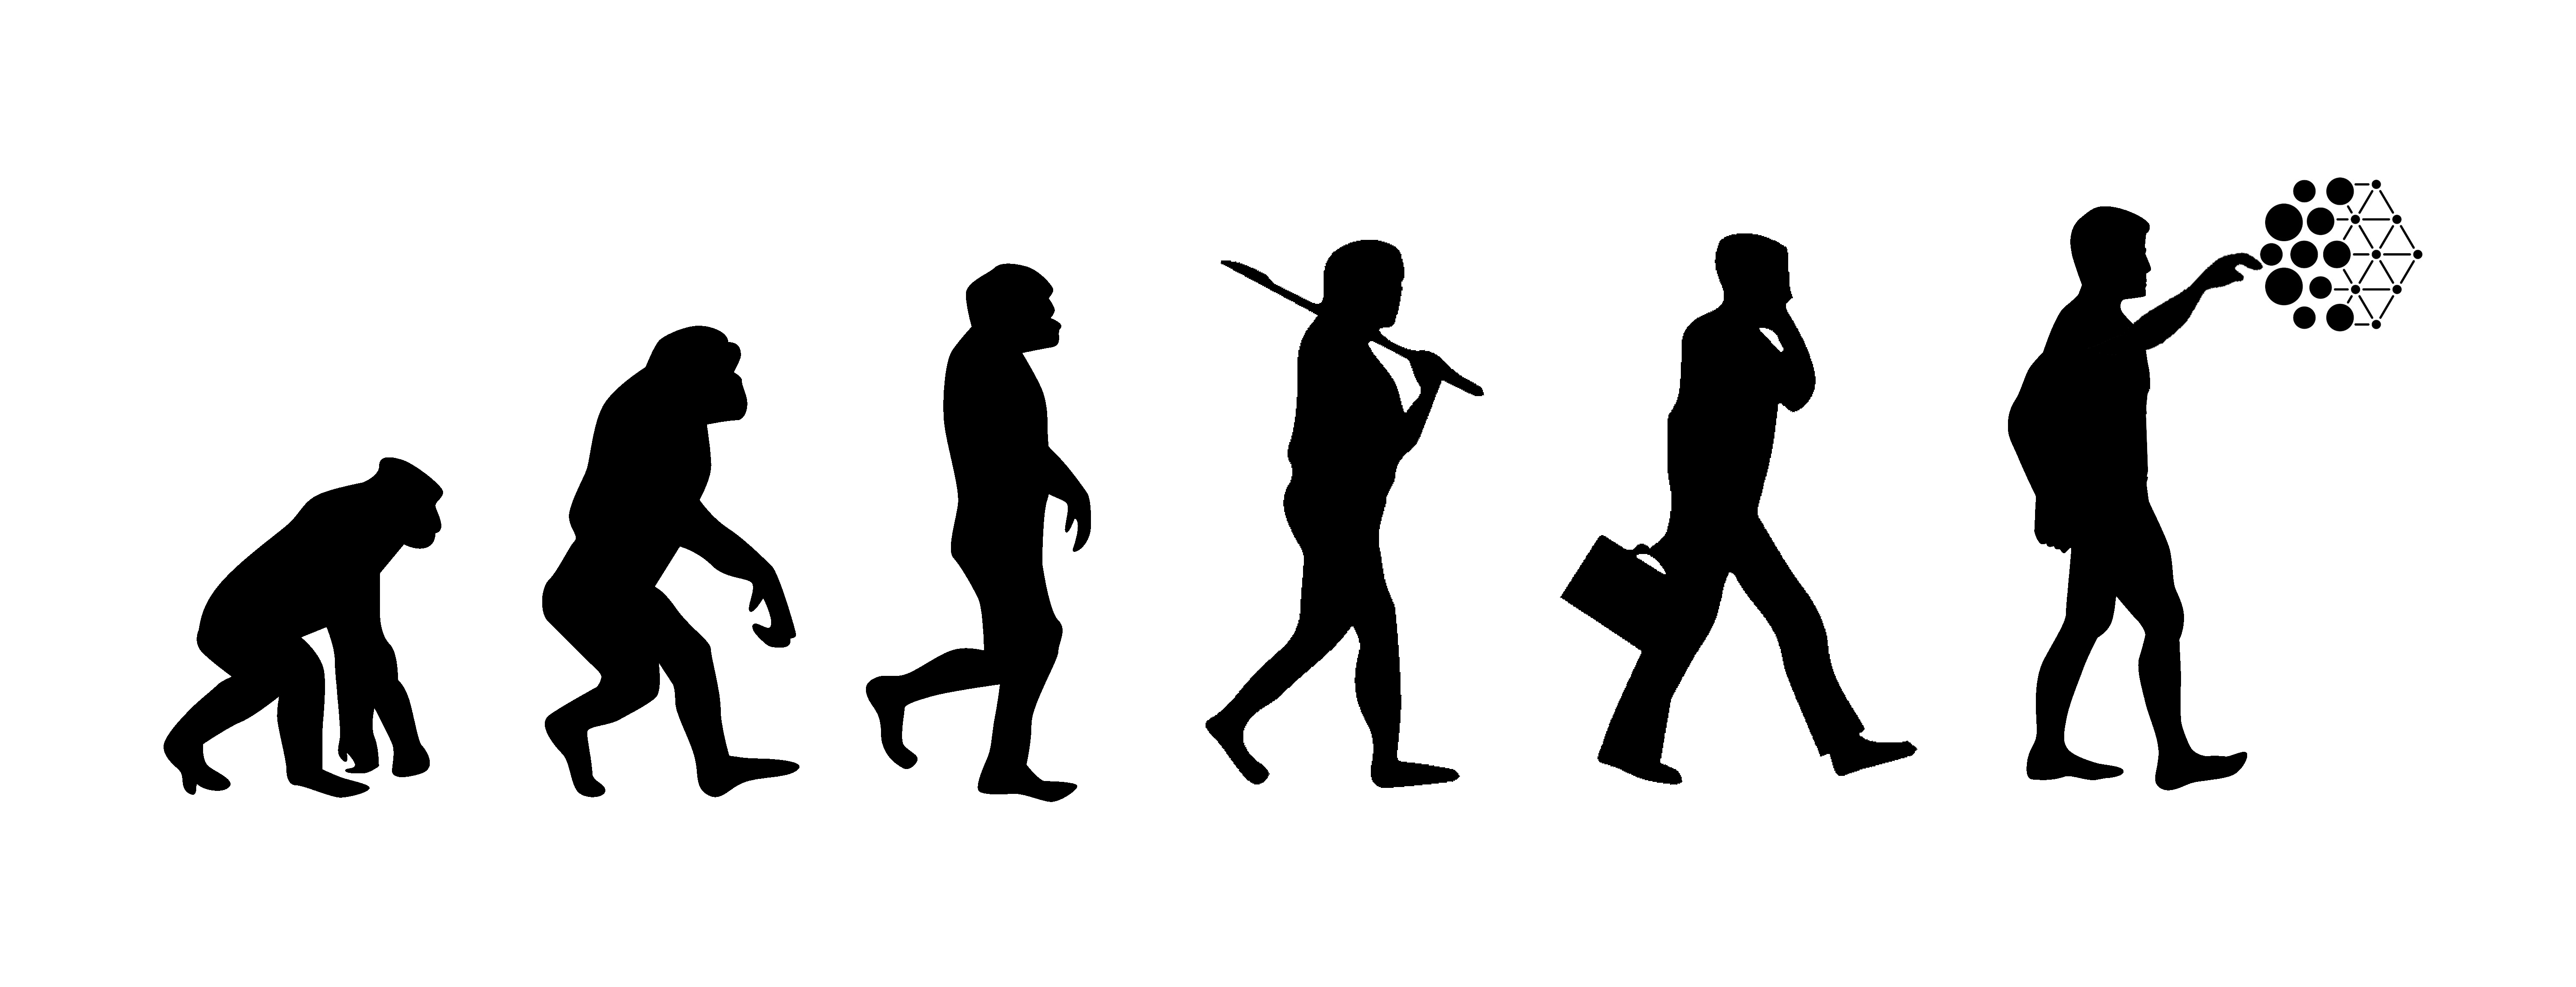
\includegraphics[width=0.90\textwidth]{../figures/evolution.png}
% 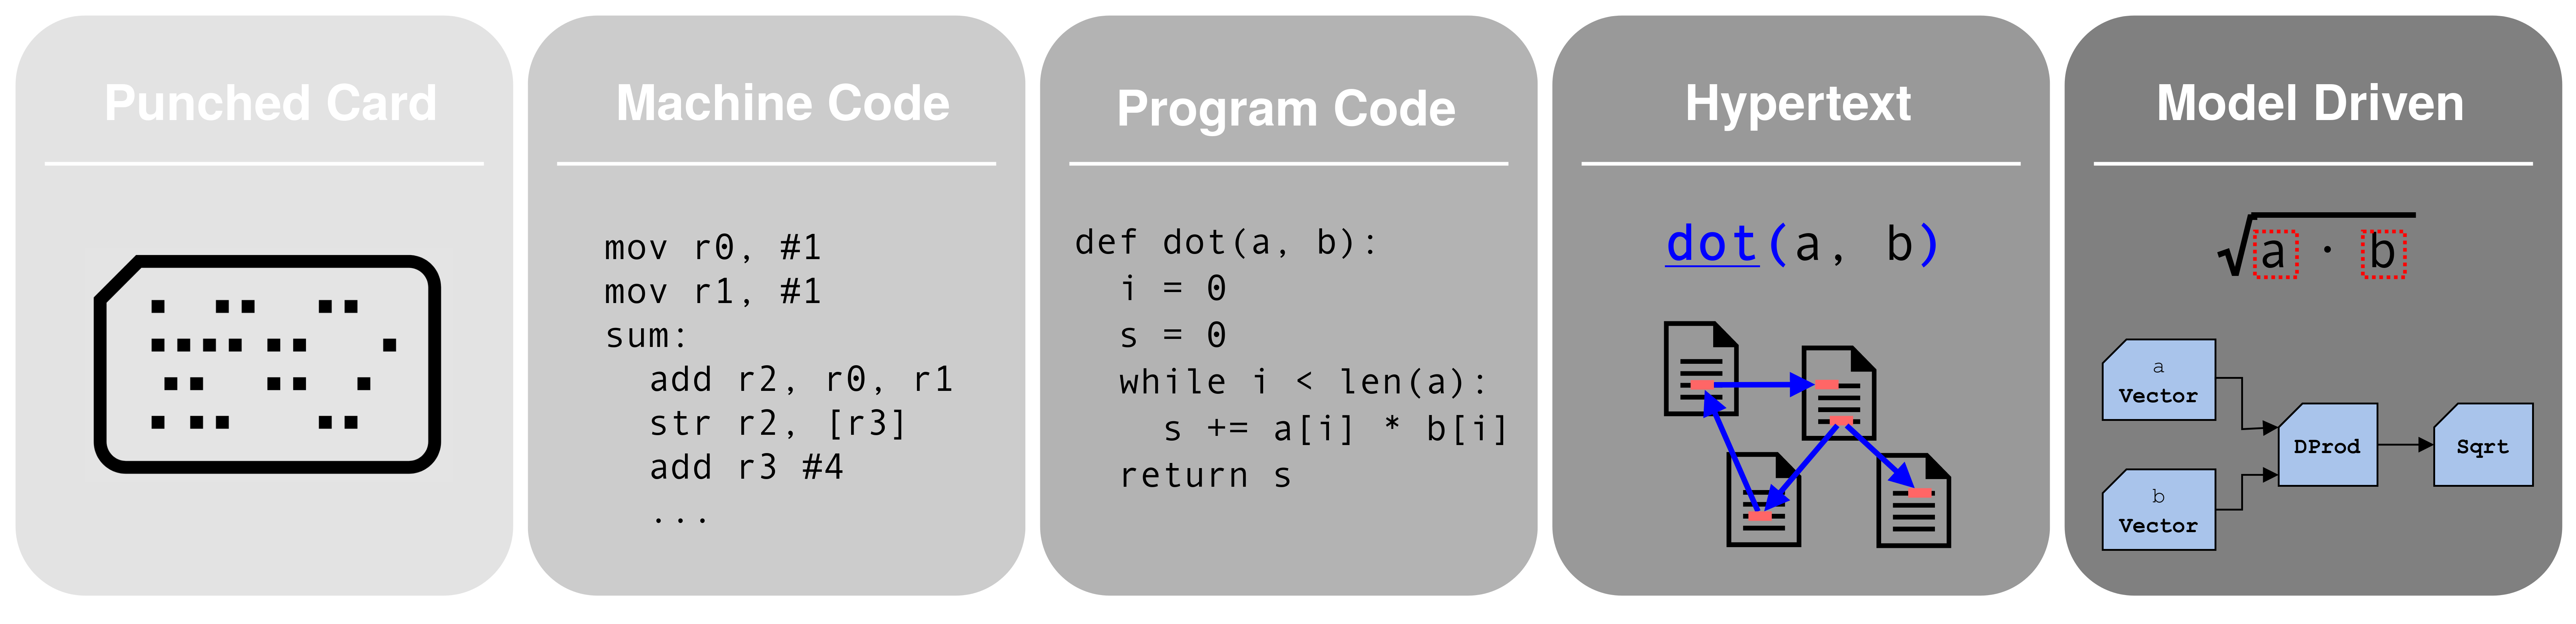
\includegraphics[width=0.90\textwidth]{../figures/progress_in_program.png}
% \caption{The evolution of code. A gauche, les langues qui obligent l'utilisateur à s'adapter à la machine. À droite, on trouve des représentations de plus en plus souples du code source.}
% \label{fig:evolution_of_programming}
%\end{figure}
%
%A l'aube de l'ère de l'information, notre espèce est à l'aube d'une nouvelle ère de l'adolescence. Les mêmes organes autrefois développés pour la planification des mouvements dans l'espace de configuration euclidienne sont utilisés d'une manière jamais imaginée par nos géniteurs. À cette époque, une seule vie et les esprits les plus brillants de notre génération suffisent à peine pour franchir les frontières de la connaissance humaine. Les ingénieurs doivent consacrer la première moitié de leur carrière intellectuelle à l'acquisition de connaissances. Les scientifiques peinent pendant des années à construire les infrastructures nécessaires à la réalisation d'expériences simples. Si nous devons faire pousser des branches plus hautes de notre arbre de la connaissance, envoyer des racines pivotantes dans des puits de compréhension plus profonds, les dotations de la nature ne peuvent pas nous mener bien loin. Si l'humanité veut atteindre son plein potentiel dans le temps qui lui est imparti, sa population croissante de travailleurs de la connaissance aura besoin d'un nouvel ensemble d'outils pour transcender la complexité croissante de l'innovation.
%
%Chaque étape du processus de création de connaissances est lourde d'une complexité fortuite découlant de l'acquisition et de la maîtrise d'une expertise spécifique à un domaine, de la découverte et du transfert de connaissances existantes, du processus de conception et de prototypage, de la validation et de la vérification de ces conceptions, et enfin de l'entretien et des aspects opérationnels de la mise en production des systèmes de connaissances. L'ensemble de cette entreprise requiert une quantité énorme de ressources humaines pour pouvoir chorégraphier efficacement. Dans l'industrie de l'information, ces personnes sont souvent appelées \textit{architectes}, \textit{ingénieurs}, \textit{développeurs}, \textit{programmeurs}, ou simplement \textit{codeurs}.\footnote{Confirmez n'importe lequel de ces camps et ils protesteront sûrement, mais les différences sont le plus souvent exagérées.} Selon certaines enquêtes~\citep{data2018global}, leur population devrait dépasser les 61 millions d'ici 2020, sans parler de la gestion et de l'administration de leurs activités sur le lieu de travail.
%
\citet{kernighan1976software} introduit d'abord le terme \textit{outils logiciels} dans le contexte des utilitaires en ligne de commande Unix, à peu près dans le même esprit que les outils proposés dans cette thèse. \citet{thrun2000towards, erez2015simulation} développer des outils basés sur le langage et la simulation pour le développement de la robotique dans le même esprit. D'une manière générale, nous considérons tout logiciel qui aide les utilisateurs engagés dans l'activité d'écriture de programmes informatiques, comme un \textit{outil de programmation}.

Dans cette thèse, nous faisons de petits pas vers la réduction de la complexité de la programmation des systèmes intelligents, grâce à des outils de programmation. Tout d'abord, nous présentons un plugin pour la construction d'applications robotiques (\autoref{ch:hatchery}). Ensuite, nous décrivons un langage spécifique à un domaine pour écrire des programmes différenciables (\autoref{ch:kotlingrad}). En utilisant notre DSL (\autoref{ch:difftest}) comme véhicule, nous développons un cadre contradictoire pour tester les programmes différentiables et démontrons empiriquement son efficacité par rapport à une méthode d'échantillonnage probabiliste. Nous discutons ensuite d'une solution basée sur un conteneur pour la reproduction de programmes robotiques, et plus largement de tout système logiciel embarqué ayant des capacités visuomotrices (\autoref{ch:ducker}). Enfin, dans \autoref{ch:conclusion} nous proposons quelques réflexions et prévisions pour l'avenir de la programmation des systèmes intelligents. Il reste encore beaucoup de travail à faire. Nous pensons que l'avenir est brillant et nous espérons que ceux qui se consacrent à sa construction s'inspireront des orientations proposées ici.

\clearpage

\section{Iconographie}

Tout au long de cette thèse, l'iconographie suivante est utilisée pour indiquer:
%
\begin{enumerate}
    \item[] \inlineimg{../figures/laptop_icon.png} & Commandes shell destinées à un ordinateur, ou sortie dérivée de celui-ci. \\
    \vspace{-0.2cm}\item[] \inlineimg{../figures/bnf_file.png} & Références GrammarKit \inline{.bnf}~\footnote{GrammarKit usage notes: \url{https://github.com/JetBrains/Grammar-Kit/blob/master/HOWTO.md}} \\
    \vspace{-0.2cm}\item[] \inlineimg{../figures/docker_icon.jpg} & Soit \inline{Dockerfile}~\footnote{Références Dockerfile: \url{https://docs.docker.com/engine/reference/builder/}} ou Docker Compose~\footnote{Compose la référence du fichier: \url{https://docs.docker.com/compose/compose-file/}} syntaxe. \\
    \vspace{-0.2cm}\item[] \inlineimg{../figures/raspi_icon.png} & Commandes shell qui doivent être exécutées sur un Raspberry Pi. \hspace{-.08em}\footnote{Raspberry Pi: \url{https://www.raspberrypi.org/}} \\
    \vspace{-0.2cm}\item[] \inlineimg{../figures/duckietown.png} & Commandes shell Duckietown (\inline{dts}).\hspace{-.08em}\footnote{Duckietown Shell: \url{https://github.com/duckietown/duckietown-shell-commands}} \\
    \vspace{-0.2cm}\item[] \inlineimg{../figures/launch_icon.png} & Fichiers roslaunch \inline{.launch}.\hspace{-.08em}\footnote{ROSLaunch XML: \url{https://wiki.ros.org/roslaunch/XML}} \\
    \vspace{-0.2cm}\item[] \inlineimg{../figures/python_icon.png} & Code source de Python.\hspace{-.08em}\footnote{Documentation Python: \url{https://www.python.org/doc/}} \\
    \vspace{-0.2cm}\item[] \inlineimg{../figures/kotlin_file.png} & Code source de Kotlin.\hspace{-.08em}\footnote{Documentation Kotlin: \url{https://kotlinlang.org/docs/reference/}}
\end{enumerate}